%
%===============>>  ГРУППА 11-2 МОДУЛЬ 8  <<=============
%
\setmodule{8}

%BEGIN_FOLD % ====>>_____ Занятие 1 _____<<====
\begin{class}[number=1]
	\begin{listofex}
		\item
		\begin{minipage}[t]{\bodywidth}
			На рисунке изображён график функции \[ f(x)=a \cos{x}+b \] Найдите \(a\).
		\end{minipage}
		\hspace{0.02\linewidth}
		\begin{minipage}[t]{\picwidth}
			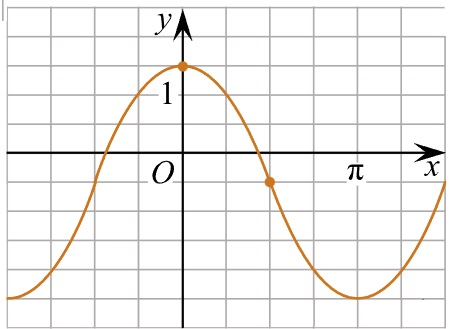
\includegraphics[align=t, width=\linewidth]{\picpath/MECGERM6H3-1}
		\end{minipage}
		%?
		\item
		\begin{minipage}[t]{\bodywidth}
			На рисунке изображён график функции \[ f(x)=a \tg{x}+b \] Найдите \(a\).
		\end{minipage}
		\hspace{0.02\linewidth}
		\begin{minipage}[t]{\picwidth}
			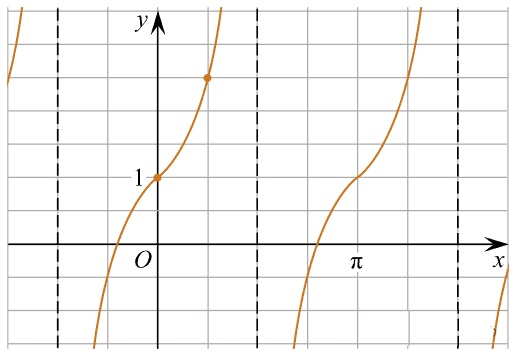
\includegraphics[align=t, width=\linewidth]{\picpath/MECGERM6H3-2}
		\end{minipage}
		\item %1 параболы
		\begin{minipage}[t]{\bodywidth}
			На рисунке изображены графики функций \(f(x) = 4x^2-25x+41 \) и \( g(x)=ax^2+bx+c \), которые пересекаются в точках \(A\) и \(B\). Найдите абсциссу точки \(B\).
		\end{minipage}
		\hspace{0.02\linewidth}
		\begin{minipage}[t]{\picwidth}
			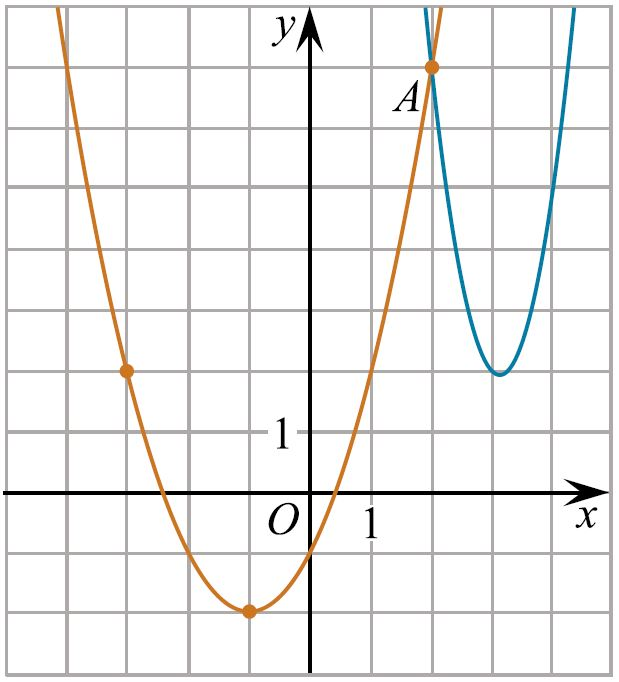
\includegraphics[align=t, width=\linewidth]{../pics/G112M3C1-10}
		\end{minipage}
		\item %1 LOGARIFM
		\begin{minipage}[t]{\bodywidth}
			На рисунке изображен график функции \(f(x) = b+\log_ax \). Найдите \(f(32)\).
		\end{minipage}
		\hspace{0.02\linewidth}
		\begin{minipage}[t]{\picwidth}
			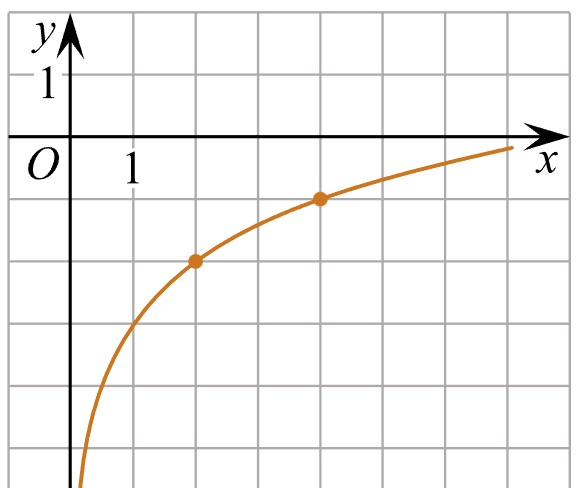
\includegraphics[align=t, width=\linewidth]{../pics/G111M8L1-1}
		\end{minipage}
		%\item %1 s golovi
		%\begin{minipage}[t]{\bodywidth}
		%	На рисунке изображен график функции \(f(x) = \dfrac{ x^2 }{ a }+bx+c \), где числа \(a, b, c\) --- целые. Найдите значение \(f(3,5)\).
		%\end{minipage}
		%\hspace{0.02\linewidth}
		%\begin{minipage}[t]{\picwidth}
		%	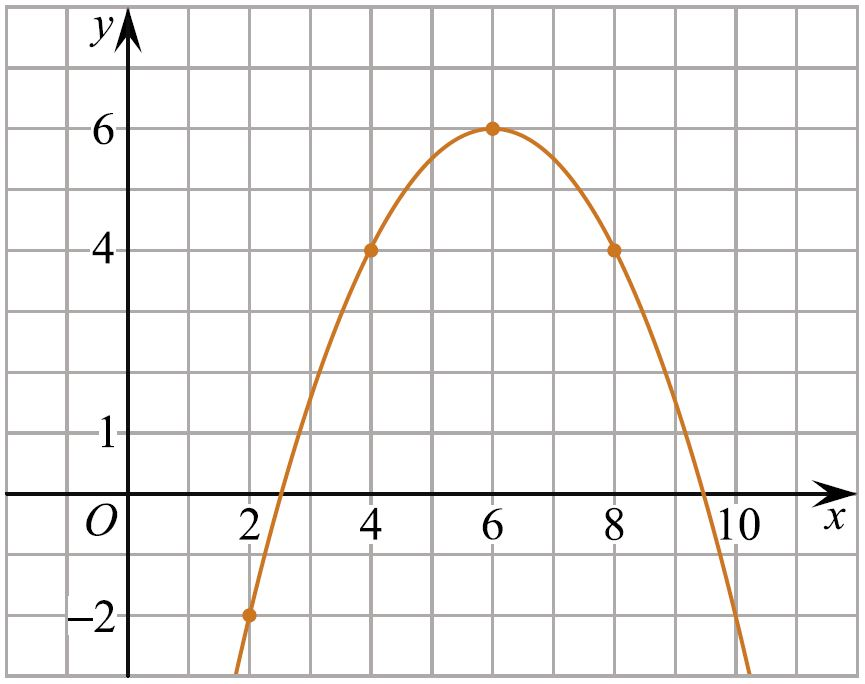
\includegraphics[align=t, width=\linewidth]{../pics/G112M3C1-6}
		%\end{minipage}
		\item Решите неравенства: %c193 23 24 27 28 a
		\begin{tasks}(2)
			\task \( \sqrt[4]{x^2-24x} \le 3 \)
			\task \( \sqrt[28]{8x-x^2-15} < 1 \)
			\task \( \sqrt[]{x^2-2x-15} < 3 \)
			\task \( \sqrt[]{3x^2-14x+51} \ge 6 \)
		\end{tasks}
		\item Решите неравенства:
		\begin{tasks}(1)
			\task \( \sqrt[]{x^4-2x+6} \ge x \)
			\task \( \sqrt[]{5x^4-28x^2+16} \ge x^2+4 \)
		\end{tasks}
		\newpage
		\item Решите неравенства: %с289 1 2 3 5 6 8
		\begin{tasks}(2)
			\task \( 4^{\tfrac{5}{x}} \ge 64 \)
			\task \( \left( \dfrac{ 1 }{ 3 } \right)^{\tfrac{ 3x+2 }{ 1-x }} < 81 \)
			
			\task \( 3^x \cdot \left( \dfrac{ 1 }{ 81 } \right)^{2x+3} < 9 \)
			\task \( 4^{3x-2}+4^{3x-1} \le 80 \)
			\task \( 5^{x-3}+5^{x-2}+5^{x-1} \ge 155 \)
			\task \( (0,2)^{\tfrac{x^2+11x+49}{2x-9}} \ge 5 \)
		\end{tasks}
	\end{listofex}
\end{class}
%END_FOLD

%BEGIN_FOLD % ====>>_____ Занятие 2 _____<<====
\begin{class}[number=2]
	\begin{listofex}
		\item Решить неравенство: 
		\[ 5^x+\dfrac{125}{5^x-126}\ge 0. \]
		\item Решить неравенство:
		\[ \dfrac{2}{5^x+75} \ge \dfrac{1}{5^x-25} \]
		\item Решить неравенство:
		\[ 16^{\tfrac{1}{x}-1}-4^{\tfrac{1}{x}-1}-2 \ge 0 \]
		\item Решить неравенство:
		\[ \dfrac{1}{2^x-1}+\dfrac{4^{x+\tfrac{1}{2}}-2^{x+5}+4}{2^x-16} \ge 2^{x+1} \]
		\item Решить неравенство:
		\[ 27\cdot45^x-27^{x+1}-12\cdot15^x+12\cdot9^x+5^x-3^x \le 0  \]
		\item Решить неравенство:
		\[ 2^{x+1}+\dfrac{9}{x}-\dfrac{3\cdot2^x}{x}\ge 6 \]
		\item Решить неравенство:
		\[ \dfrac{9^x+2 \cdot 3^x-117}{3^x-27} \le 1 \]
		\item Решить неравенство: \[ \dfrac{ 3^{|x^2-2x-1|}-9}{ x } \ge 0 \]
		
		
		\item Решить неравенство: \[ 64^{x^2-3x+20}-0,125^{2x^2-6x-200} \le 0 \]
		\item Решить неравенство: \[ 4^{x^2+x-3}-0,5^{2x^2-6x-2} \le 0 \]
	\end{listofex}
\end{class}
%END_FOLD

%BEGIN_FOLD % ====>>_ Домашняя работа 1 _<<====
\begin{homework}[number=1]
	\begin{listofex}
		\item Решите неравенства: %c192 n 25 26 27 28 b /c289 1 2 4 5 b
		\begin{tasks}(2)
			%\task \( \sqrt[3]{9x-x^2} \le 2 \)
			%\task \( \sqrt[]{x^2-25} \le 12 \)
			%\task \( \sqrt[]{x^2-4x-5} < 4 \)
			%\task \( \sqrt{4x^2-29x+61} \ge 3 \)
			%\task \( 3^{\tfrac{ 4 }{ x }} \ge 27 \)
			%\task \( 0,5^{\tfrac{ 3x-2 }{ 3-x }}<16 \)
			%\task \( \left( \dfrac{ 1 }{ 3 } \right)^{\tfrac{ 4x-1 }{ x-5 }} > 81^{\tfrac{ x-2 }{ x+5 }} \)
			%\task \( 6^x \cdot \left( \dfrac{ 1 }{ 36 } \right)^{5x+3} < 6 \)
			\task \( \dfrac{ 9^x-3^x-90 }{ 3^x-82 } \le 1 \)
			\task \( 2^{2x-1}-7 \cdot 2^{x-1}+5 \le 0 \)
			\task \( 2^x+80 \cdot 2^{4-x} \le 261 \)
			\task \( 2^{2x+4}-16 \cdot 2^{x+3}-2^{x+1}+16 \le 0 \)
			\task \( 6^x-4 \cdot 3^x-2^x+4 \le 0 \)
			\task \( 4^{x^2+x-3}-0,5^{2x^2-6x-2} \le 0 \)
		\end{tasks}
		%trigon10 8
		%\item
		%\begin{minipage}[t]{\bodywidth}
		%	На рисунке изображён график функции вида \[ f(x)= a\cos \left( \dfrac{ \pi x }{ b }+c \right)+d, \] где \(a,b,c, d\) --- целые. Найдите \(f\left( -\dfrac{ 22 }{ 3 } \right)\).
		%\end{minipage}
		%\hspace{0.02\linewidth}
		%\begin{minipage}[t]{\picwidth}
		%	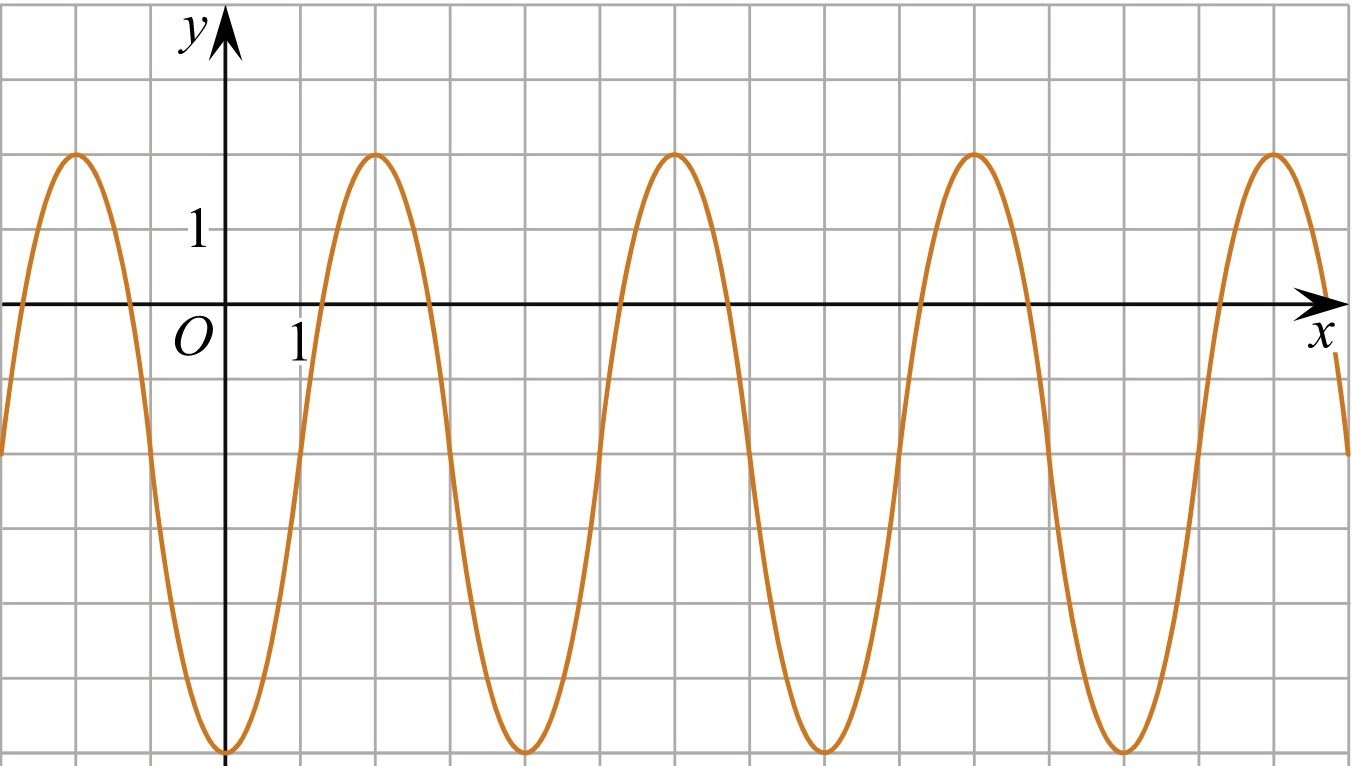
\includegraphics[align=t, width=\linewidth]{\picpath/G112M8H1-1}
		%\end{minipage}
	\end{listofex}
\end{homework}
%END_FOLD

%BEGIN_FOLD % ====>>_____ Занятие 3 _____<<====
\begin{class}[number=3]
	\begin{listofex}
		%11.1v2v3 po 3
		\item Найдите точку максимума функции \( y=x^3-48x+17 \).
		\item Найдите наименьшее значение функции \( y=x^3-27 \) на отрезке \([0;4]\).
		\item Найдите наибольшее значение функции \( y=x^3-3x+4 \) на отрезке \([-2;0]\).
		%1-4 analog 282861
		\item Найдите наименьшее значение функции \( y=(x+3)^2(x+5)-1 \) на отрезке \([-4;-1]\).
		\item Найдите наименьшее значение функции \( y=(x-7)^2(x+6) \) на отрезке \([-1;20]\).
		\item Найдите наименьшее значение функции \( y=(x-8)^2(x-1)+10 \) на отрезке \([6;14]\).
		\item Найдите наибольшее значение функции \( y=(x-2)^2(x-4)+5 \) на отрезке \([1;3]\).
		\item Найдите точку максимума функции \( y=-\dfrac{ x^2+289 }{ x } \).
		%\item Найдите точку минимума функции \( y=-\dfrac{ x^2+1 }{ x } \).
		\item Найдите наименьшее значение функции \( y=\dfrac{x^2+25  }{ x } \) на отрезке \([1;10]\).
		\item Найдите наименьшее значение функции \( y=(x-8)e^{x-7} \) на отрезке \([6;8]\).
		\item Найдите точку минимума функции \( y=(x+16)e^{x-16} \).
		\item Найдите точку максимума функции \( y=(9-x)e^{x+9} \).
		
		
		%G111M5L2
		%\item
		%\begin{minipage}[t]{\bodywidth}
		%	На рисунке изображен график функции \( y = f(x)\), определенной на интервале \((-5; 5)\). Найдите количество точек, в которых касательная к графику функции параллельна прямой \(y  =  6\) или совпадает с ней.
		%\end{minipage}
		%\hspace{0.02\linewidth}
		%\begin{minipage}[t]{\picwidth}
		%	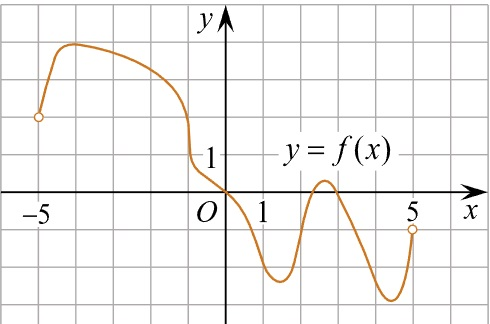
\includegraphics[align=t, width=\linewidth]{\picpath/G111M5L2-1}
		%\end{minipage}
		%\item
		%\begin{minipage}[t]{\bodywidth}
		%	На рисунке изображен график производной функции \(f(x)\), определенной на интервале \((-10; 2)\). Найдите количество точек, в которых касательная к графику функции \(f(x)\) параллельна прямой \(y = -2x - 11\) или совпадает с ней.
		%\end{minipage}
		%\hspace{0.02\linewidth}
		%\begin{minipage}[t]{\picwidth}
		%	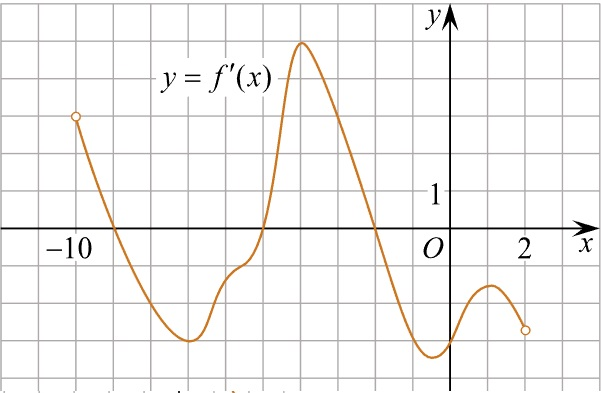
\includegraphics[align=t, width=\linewidth]{\picpath/G111M5L2-2}
		%\end{minipage}
		%G111M5L2
		\item
		\begin{minipage}[t]{\bodywidth}
			На рисунке изображен график производной функции \(f(x)\) , определенной на интервале \( (-6;6) \) . Найдите промежутки возрастания функции \(f(x)\) . В ответе укажите сумму целых точек, входящих в эти промежутки.
		\end{minipage}
		\hspace{0.02\linewidth}
		\begin{minipage}[t]{\picwidth}
			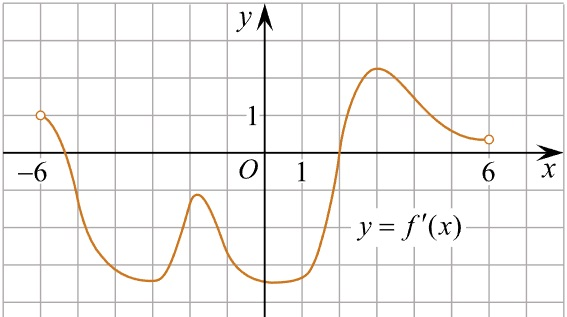
\includegraphics[align=t, width=\linewidth]{\picpath/G111M5L2-3}
		\end{minipage}
		\item
		\begin{minipage}[t]{\bodywidth}
			На рисунке изображен график функции \(y = f(x)\), определенной на интервале \((-6; 8)\). Определите количество целых точек, в которых производная функции положительна.
		\end{minipage}
		\hspace{0.02\linewidth}
		\begin{minipage}[t]{\picwidth}
			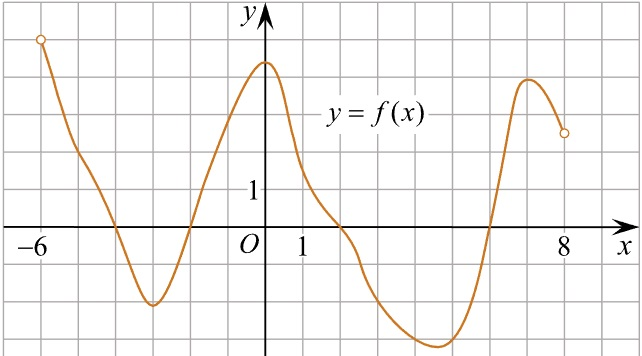
\includegraphics[align=t, width=\linewidth]{\picpath/G111M5L2-4}
		\end{minipage}
		%525690
		\item
		\begin{minipage}[t]{\bodywidth}
			На рисунке изображены график функции \(y=f(x)\) и касательная к этому графику, проведённая в точке \(x_0\). Уравнение касательной показано на рисунке. Найдите значение производной функции \(g(x)=-7f(x)+21x+\dfrac{ 1 }{ 441 }\) в точке \(x_0\).
		\end{minipage}
		\hspace{0.02\linewidth}
		\begin{minipage}[t]{\picwidth}
			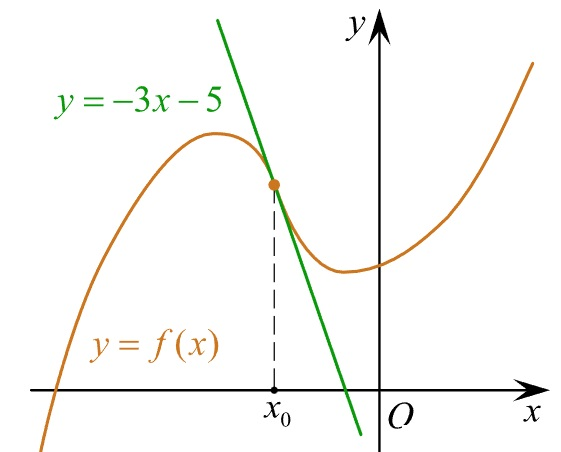
\includegraphics[align=t, width=\linewidth]{\picpath/G112M8C3-1}
		\end{minipage}
		%525702
		\item
		\begin{minipage}[t]{\bodywidth}
			На рисунке изображены график функции \(y=f(x)\) и касательная к этому графику, проведённая в точке \(x_0\). Уравнение касательной показано на рисунке. Найдите значение производной функции \(g(x)=-5f(x)-\dfrac{ 2 }{ 11 }x+\ln3\) в точке \(x_0\).
		\end{minipage}
		\hspace{0.02\linewidth}
		\begin{minipage}[t]{\picwidth}
			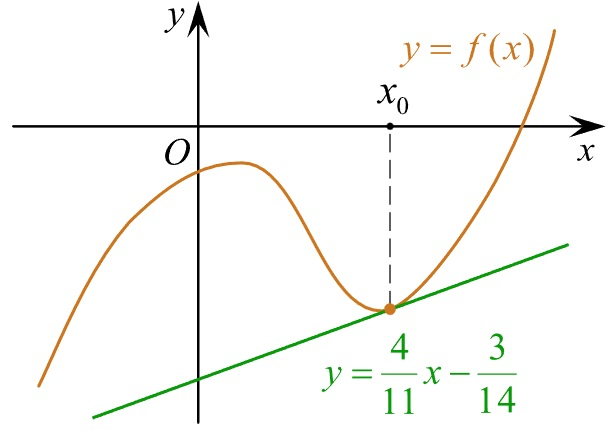
\includegraphics[align=t, width=\linewidth]{\picpath/G112M8C3-2}
		\end{minipage}
		%525691
		\item
		\begin{minipage}[t]{\bodywidth}
			На рисунке изображены график функции \(y=f(x)\) и касательная к этому графику, проведённая в точке \(x_0\). Уравнение касательной показано на рисунке. Найдите значение производной функции \(g(x)=(f'(x)-0,5)\cdot 6\) в точке \(x_0\).
		\end{minipage}
		\hspace{0.02\linewidth}
		\begin{minipage}[t]{\picwidth}
			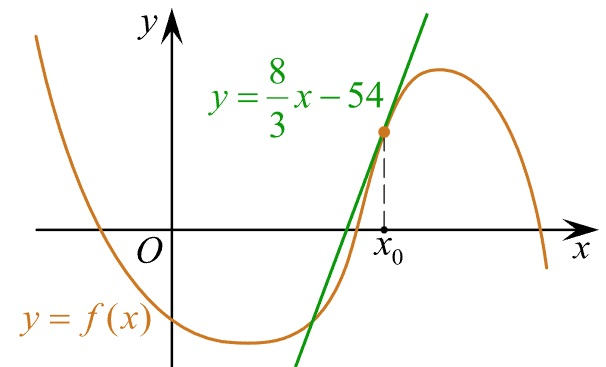
\includegraphics[align=t, width=\linewidth]{\picpath/G112M8C3-3}
		\end{minipage}
		%525703
		\item
		\begin{minipage}[t]{\bodywidth}
			На рисунке изображены график функции \(y=f(x)\) и касательная к этому графику, проведённая в точке \(x_0\). Уравнение касательной показано на рисунке. Найдите значение производной функции \(g(x)=f'(x)-f(x)+3\) в точке \(x_0\).
		\end{minipage}
		\hspace{0.02\linewidth}
		\begin{minipage}[t]{\picwidth}
			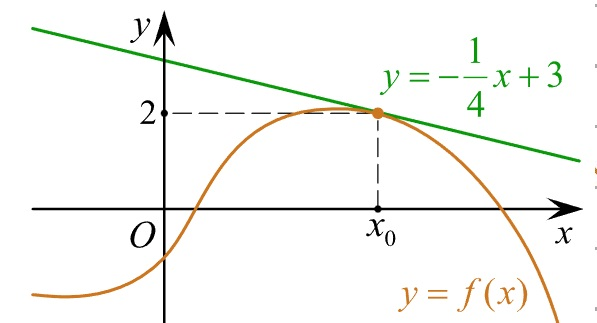
\includegraphics[align=t, width=\linewidth]{\picpath/G112M8C3-4}
		\end{minipage}
		\item
		\begin{minipage}[t]{\bodywidth}
			На рисунке изображены графики функций \(f(x)=5x+9\) и \( g(x)=ax^2+bx+c \), которые пересекаются в точках \(A\) и \(B\). Найдите абсциссу точки \(B\).
		\end{minipage}
		\hspace{0.02\linewidth}
		\begin{minipage}[t]{\picwidth}
			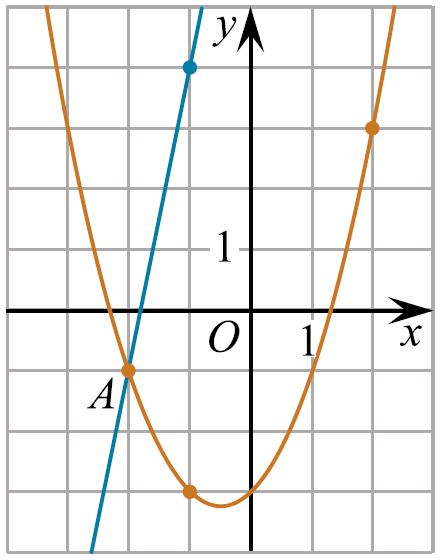
\includegraphics[align=t, width=\linewidth]{\picpath/G112M3C1-9}
		\end{minipage}
		
		\item
		\begin{minipage}[t]{\bodywidth}
			На рисунке изображен график функции \( f(x)=\dfrac{k}{x}+a \). Найдите, при каком значении \( x \) значение функции будет равно \( 0,8 \).
		\end{minipage}
		\hspace{0.02\linewidth}
		\begin{minipage}[t]{\picwidth}
			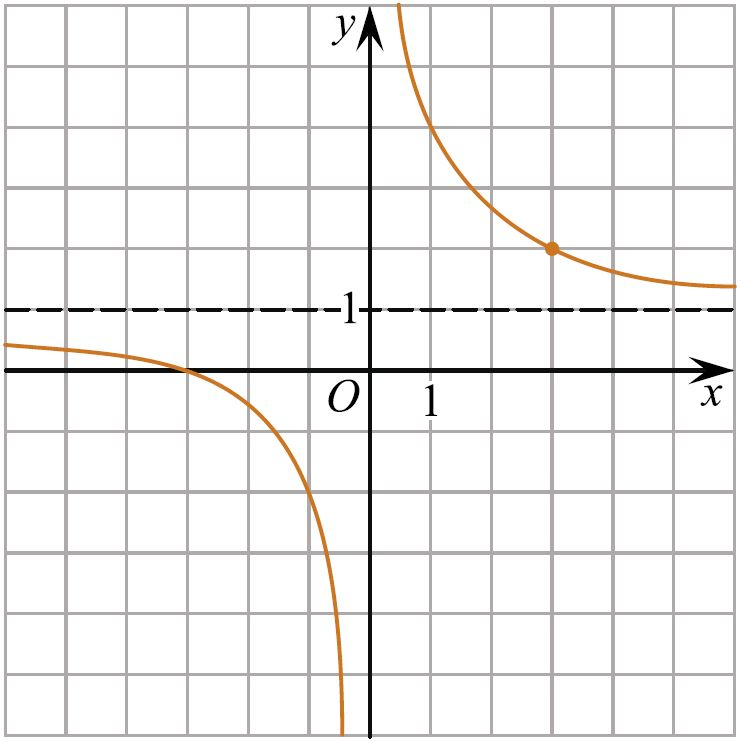
\includegraphics[align=t, width=\linewidth]{\picpath/G112M3C2-5}
		\end{minipage}
		\item %1 LOGARIFM
		\begin{minipage}[t]{\bodywidth}
			На рисунке изображен график функции \(f(x) = b+\log_ax \). Найдите \(f(32)\).
		\end{minipage}
		\hspace{0.02\linewidth}
		\begin{minipage}[t]{\picwidth}
			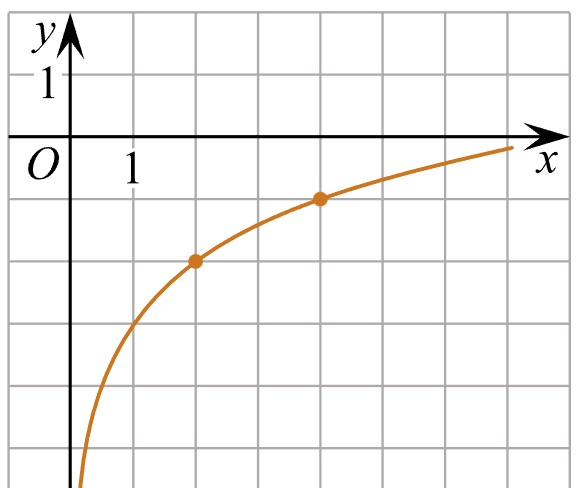
\includegraphics[align=t, width=\linewidth]{../pics/G111M8L1-1}
		\end{minipage}
	\end{listofex}
\end{class}
%END_FOLD

%BEGIN_FOLD % ====>>_____ Занятие 4 _____<<====
\begin{class}[number=4]
	\begin{listofex}
		\item Решите неравенства: %c298 a 1 2 4 6 7 8 9 10
		\begin{tasks}(2)
			\task \( \log_x<2 \)
			\task \( \log_3x\le3 \)
			\task \( \log_{0,123}x \le 0 \)
			\task \( \log_{0,04}x \ge -1 \)
			\task \( \log_5 (4x+5) < 3 \)
			\task \( \log_{0,1}(3x+25)<-2 \)
			\task \( \log_{\tfrac{2}{7}}(2x-2,5)\le -1 \)
			\task \( \log_3 (10x-19)>4 \)
		\end{tasks}
	\end{listofex}
\end{class}
%END_FOLD

%BEGIN_FOLD % ====>>_ Домашняя работа 2 _<<====
\begin{homework}[number=2]
	\begin{listofex}
		\item Домашняя работа 2
	\end{listofex}
\end{homework}
%END_FOLD

%BEGIN_FOLD % ====>>_____ Занятие 5 _____<<====
\begin{class}[number=5]
	\begin{listofex}
		\item Занятие 5
	\end{listofex}
\end{class}
%END_FOLD

%BEGIN_FOLD % ====>>_____ Занятие 6 _____<<====
\begin{class}[number=6]
	\begin{listofex}
		\item Занятие 6
	\end{listofex}
\end{class}
%END_FOLD

%BEGIN_FOLD % ====>>_ Домашняя работа 3 _<<====
\begin{homework}[number=3]
	\begin{listofex}
		\item Домашняя работа 3
	\end{listofex}
\end{homework}
%END_FOLD

%BEGIN_FOLD % ====>>_____ Занятие 7 _____<<====
\begin{class}[number=7]
	\title{Подготовка к проверочной}
	\begin{listofex}
		\item Занятие 7
	\end{listofex}
\end{class}
%END_FOLD

=%BEGIN_FOLD % ====>>_ Проверочная работа _<<====
\begin{exam}
	\begin{listofex}
		\item Проверочная
	\end{listofex}
\end{exam}
%END_FOLD

%\item Решите неравенства: %192 25 27 28 a
%\begin{tasks}(2)
%	\task \( \sqrt[3]{6x-x^2} \le 2 \)
%	\task \( \sqrt[]{x^2-2x-15}<3 \)
%	\task \( \sqrt[]{3x^2-14x+51} \ge 6 \)
%	\task \( \sqrt[]{x^2-144} \le 5 \)
%	\task \( \sqrt[]{x^4-2x+6} \ge x \)
%	\task \( \sqrt[]{5x^4-28x^2+16} \ge x^2+4 \)
%\end{tasks}
%\item Решите неравенства: %с289 1 2 3 5 6 8
%\begin{tasks}(2)
%	\task \( 4^{\tfrac{5}{x}} \ge 64 \)
%	\task \( \left( \dfrac{ 1 }{ 3 } \right)^{\tfrac{ 3x+2 }{ 1-x }} < 81 \)
%	
%	\task \( 3^x \cdot \left( \dfrac{ 1 }{ 81 } \right)^{2x+3} < 9 \)
%	\task \( 4^{3x-2}+4^{3x-1} \le 80 \)
%	\task \( 5^{x-3}+5^{x-2}+5^{x-1} \ge 155 \)
%	\task \( (0,2)^{\tfrac{x^2+11x+49}{2x-9}} \ge 5 \)
%\end{tasks}